\section{大型加速器実験}
加速器実験では、加速させた高エネルギーの粒子同士を衝突させることで、新たな粒子を作り出すことや、粒子同士の相互作用を観測することができる。
%また、宇宙初期の状態を模倣することもできる。
粒子の衝突点付近に検出器を設置することで、加速器によって生じたさまざまな粒子を観測することができる。検出器によって、粒子の飛跡や運動量、エネルギーをすることで、
生成された粒子の性質やその粒子と他の物質との相互作用などを調べることができる。そのような測定を通して、大型加速器実験では新粒子や新物理の探索を行っている。

現在行われている世界最大の加速器実験が、大型ハドロン衝突型加速器(LHC)実験である。
LHCは、図\ref{fg:LHC}にあるように1 周約27 kmの加速器で、真空の管パイプで光速近くまで加速させた陽子同士を衝突させることで、新粒子の探索を行っている。
LHC実験は、13.6 TeVという世界最大のエネルギーでの陽子・陽子衝突を起こすことができる。
質量が重い新粒子や高エネルギー領域での新たな物理法則の発見が期待されている。

加速器実験は、反応確率が小さい事象や質量が大きい粒子を発見するために、高輝度化と高エネルギー化を繰り返しながら発展してきた。
%反応確率が小さい事象や、超対称性粒子のような質量が非常に重い粒子を作り出すために、さらに多くのデータ量と高エネルギーの粒子の衝突
LHCはエネルギーが14 TeV、衝突頻度を上げることで、1年間で取得するデータ量がLHCの約10 倍の高輝度大型ハドロン衝突型加速器(HL-LHC)にアップグレードすることが決まっている。
また、重心系エネルギーが約27 TeVのHigh Energy LHC(HE-LHC)や重心系エネルギーが100TeVのFuture Circular Colider(FCC)も検討されている。

LHCの衝突点で行われている実験の1つにATLAS実験がある。ATLAS実験では、直径25 m、長さ46 mの円筒状のATLAS検出器を使って、陽子と陽子の衝突によって生成された粒子の測定を行っている。
衝突によって生成された粒子の再構成を行うために、ATLAS検出器の最内層に置かれている検出器を内部飛跡検出器と呼ぶ。
将来の素粒子実験では、さらなる高輝度化と高エネルギー化に伴って、
衝突点で生成される粒子の数が激増するため、それらを効率よくとらえて飛跡を再構成するために、内部飛跡検出器の改良が求められている。

\begin{figure}[h]
    \centering
    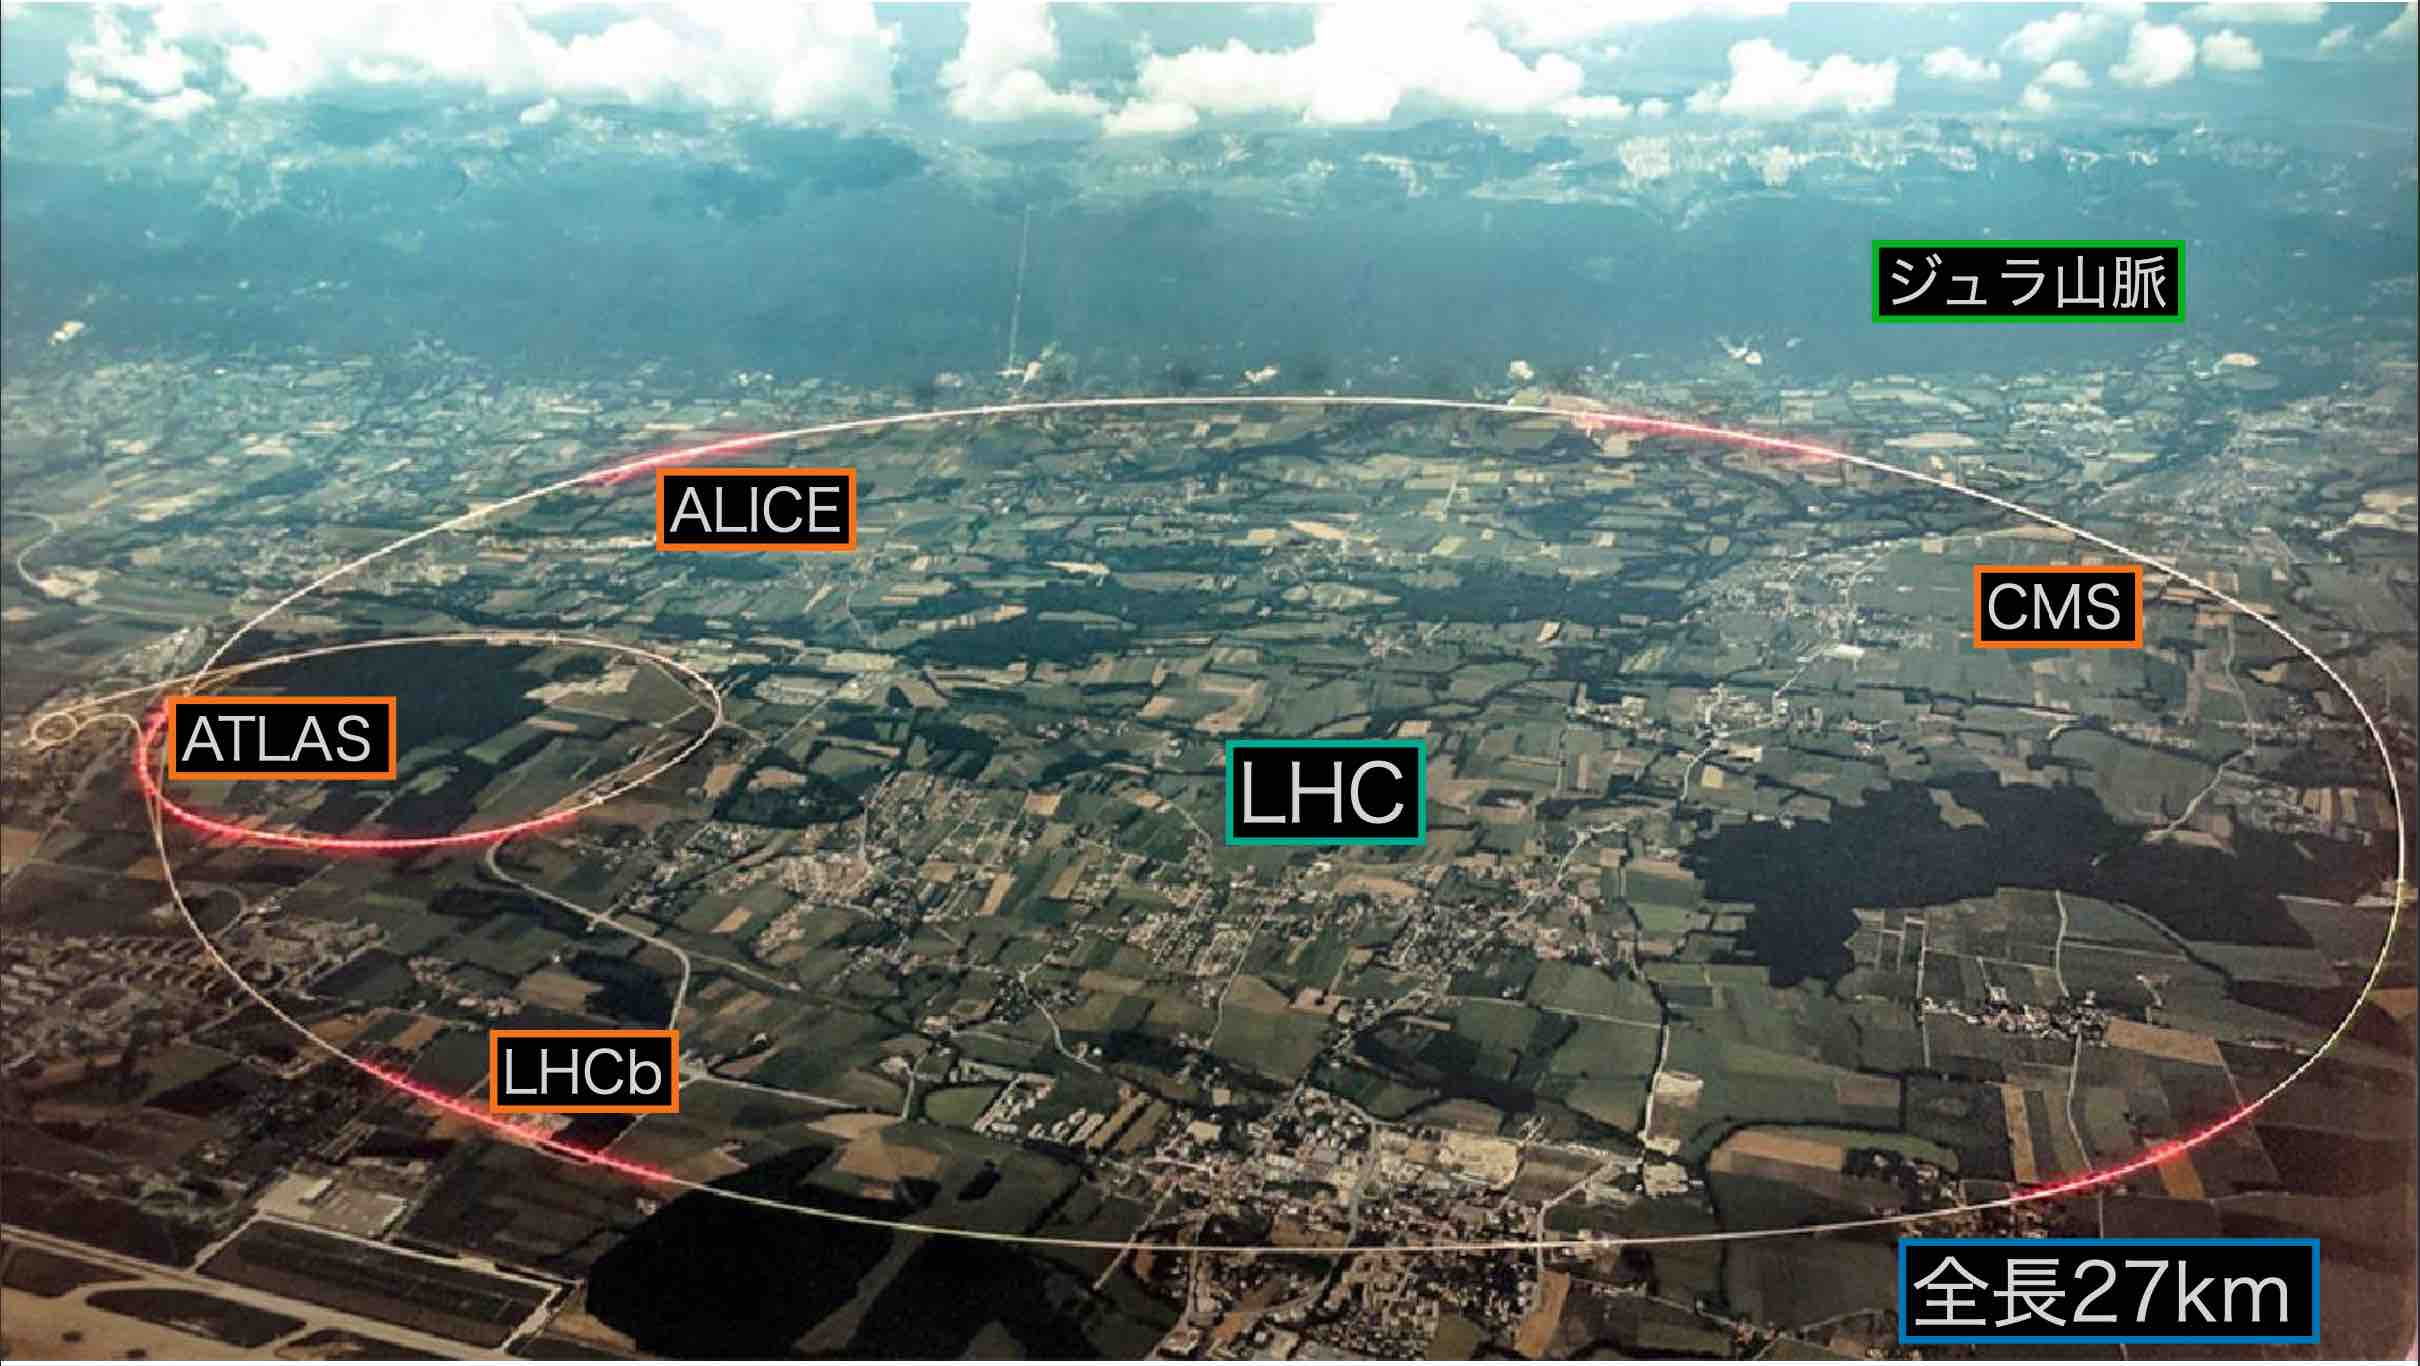
\includegraphics[width=12cm]{fig/ch1/LHC.jpg}
    \caption{Large Hadron Colider(LHC)の鳥瞰図\cite{LHCphoto}}
    \label{fg:LHC}
\end{figure}